\section{Architecture}

The following picture shows the core components and interfaces

\begin{figure}[h]
    \centering
    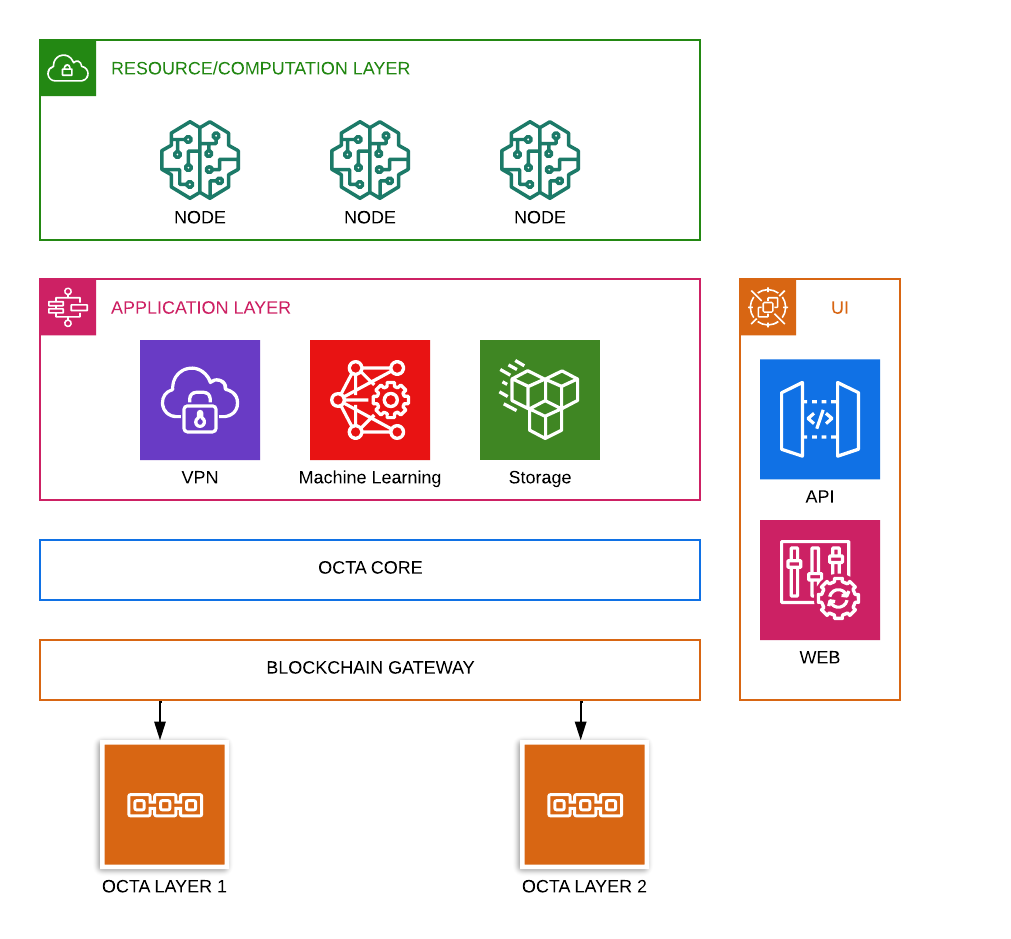
\includegraphics[width=\textwidth]{octa-arch}
    \caption{High Level Architecture}
\end{figure}

\subsection{Blockchain}
OctaSpace utilizes a Layer 1 PoW blockchain that is secured using the pirl 51\% guard technique. This security protocol provides protection against attacks on the network, making it a secure platform for users to transact on.

In addition to the Layer 1 PoW blockchain, OctaSpace also employs a Layer 2 PoA blockchain that is used to speed up transactions for billing operations. This blockchain is based on validators and is not used to secure the Layer 1 PoW blockchain.

By utilizing this Layer 2 PoA blockchain, OctaSpace is able to process a large number of transactions quickly and efficiently for billing operations such as charging users for the services they have used.

Overall, OctaSpace's use of the pirl 51\% guard and Layer 2 PoA blockchain demonstrate its commitment to security and efficiency. By employing these techniques, OctaSpace is able to provide a secure and stable platform for its users while also maintaining fast and efficient transactions for billing operations.

\newpage

\subsection{Layer 1 network}

\textbf{OCTA Layer 1} is PoW\cite{pow} blockchain network is used for the frontend user financial operations using the native coin OCTA.

Network based on go-ethereum\cite{go-ethereum} codebase with the following specification:

\begin{itemize}
    \item Block time is 15 seconds
    \item Total supply is unlimited\footnote{Total supply will be reviewed after Mahasim fork}
    \item Block reward and halving implemented according to \hyperref[sec:mp]{Monenary policy}
    \item PirlGuard is used as protection mechanism from 51\% attack
    \item Transaction fee is 21 Gwei
\end{itemize}

OctaSpace network is designed to be fair and transparent, without any premine or presale. To ensure an equitable distribution of rewards, the genesis difficulty was set at 100Gh, preventing the instant allocation of rewards.

\subsection{Layer 2 network}

This is a side chain for Layer 1 network, implemented as PoA\cite{poa} network with a set of validators.

Used for handling internal transactions for the node services its lightning-fast performance and its seamlessly handling of high-frequency, high-usage operations,
resulting in reduced operational costs, speedy transactions and a massive boost in charging operations throughput.

\subsection{Blockchain gateways}

These gateways provides unified API for \textbf{OCTA CORE} layer to give it ability work with both blockchain networks.

This API is private and not accessible outside.

\subsection{OCTA CORE and Application Layer}
The engine of our system, the compute rental manager, seamlessly handles all requests for compute rentals and communicates with the nodes and user applications to make it effortless for users to access and use the resources of connected nodes.

This layer is designed to be user-friendly, so even those without technical expertise can take advantage of the available resources with ease.

Its the core engine of our system, it's responsible for the following operations:

\begin{itemize}
    \item Communicates, monitoring and low level interaction with nodes
    \item Handle requests for computing resources
    \item Provide interface for creating services on a top of resources provided by nodes
    \item Services usage charging and billing operations
    \item Provide API for automation or integration with third party systems
    \item Fraud control
    \item Statistic and telemetry of system usage
\end{itemize}

\subsection{Resource Layer}
While the Octa Chain is very capable at processing large amounts of transactions the real aim of the project is to provide real world applications and to bridge the gap of computational owners and computational users. Octa nodes were built to accomplish this.

This layer consist of hardware(nodes) connected to the OctaSpace cloud.

Nodes are the foundation of our compute and services marketplace, providing the necessary computational power to meet the demands of tasks.

These computers are equipped with a blend of CPUs, GPUs, memory, and disk space that allows them to handle distributed workloads with ease.

The nodes are connected to the OctaSpace, which enables them to seamlessly work together to deliver optimal performance and efficiency.

The tasks and services may vary, well equipped machines with powerful GPU may performs AI/ML tasks, common machines may acts as VPN gateway, provide disk storage for services like file sharing or host applications deployed by users.

\subsection{API and UI}

To work with system the following interfaces available:

\begin{itemize}
    \item Web applicaton with user-friendly interface: \url{https://cube.octa.space}
    \item RESTful API
    \item \textbf{octactl} command-line utility that provide user friendly interface to RESTful API
\end{itemize}
